\documentclass[UTF8]{ctexart}
\pagestyle{plain}
\usepackage{amsmath}
\usepackage{amssymb}
\usepackage{cite}
\usepackage{url}
\usepackage{graphicx}
\usepackage{geometry}
\usepackage{type1cm}
\geometry{papersize = {210mm,297mm}}
\geometry{left = 3.18cm,right = 3.18cm,top = 2.54cm,bottom = 2.54cm}
\title{对张量及其特征值的理解}
\begin{document}
\fontsize{12pt}{18pt}
\selectfont
\date{}
\maketitle
\section{摘要}
通常定义张量的物理学或传统数学方法,是把张量看成一个多维数组,当变换坐标或变换基底时,其分量也会按照一定的规则变换。随着张量在各个学科中的广泛应用,我们需要将其抽象化,本文主要讨论张量的发展过程以及我个人的一些理解。\newline
{\bfseries关键词}:张量,多重线性映射,对偶空间,张量的特征值
\section{张量的历史背景}
1846年,Sir William Rowan Hamilton 引入"张量"一词,用于指代现在称为模的对象。1890年,Gregorio Ricci-Curbastro发表《绝对微分几何》,引入该词的现代意义。1900年,Tullio Levi-Civita发表《绝对微分》,张量为数学家所广知。1915年,Albert Einstein发表广义相对论,张量微积分获得更广泛的承认。
\section{张量的定义}
一个$\textbf{(m,n)}$型的张量被定义为一个多重线性映射:
$$T : \underbrace{V^* \times \cdots \times V^*}_{m \ copies} \times \underbrace{V \times \cdots \times V}_{n \ copies} \to \mathbb{R}$$
其中V是向量空间,$V^*$是对应的对偶空间。\cite{lawden1982introduction}
\subsection{多重线性映射的定义}
在线性代数中,多重线性映射是指有多个向量变量而对每个变量都是线性函数的映射。 \newline
例如:$f(x,y) = xy$为双线性映射,但是$f(x,y) = x^2$不是多重线性映射。
\subsection{对偶空间}
想要理解张量的定义必须先理解对偶空间,下文将给出定义和一种形象化的理解。
\subsubsection{对偶空间的定义}
在数学中,任何向量空间V都有其对应的对偶向量空间,由V的线性泛函构成。此对偶空间具有一般向量空间的结构。\cite{bourbaki1989algebra}
\subsubsection{对偶空间的形象化理解}
首先,假设存在一条直线$ax + by = C$,如图所示:\newline
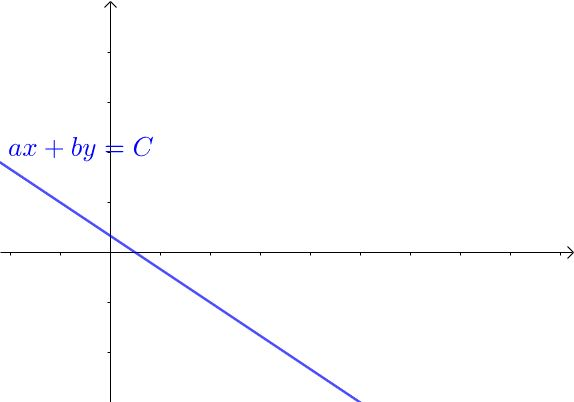
\includegraphics[width=.8\textwidth]{dual1.jpg} \newline
这时$x$和$y$为变量。若以$a$和$b$为变量,在$ax + by = C$上任取一点$A$,其坐标为$(A_x,A_y)$,画出$$A_xa + A_yb = C$$ 如下图所示:\newline
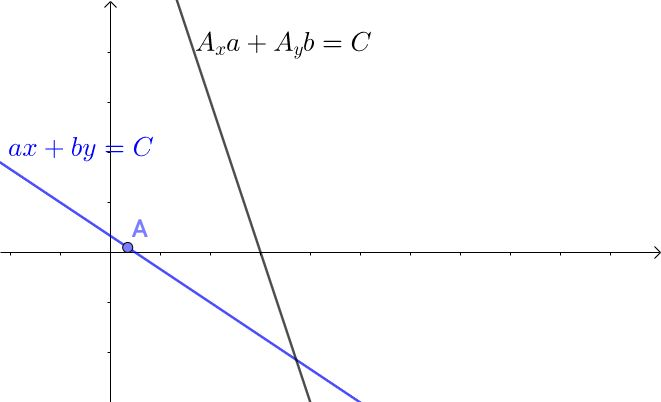
\includegraphics[width=.8\textwidth]{dual2.jpg} \newline
若$A$沿直线$ax + by = C$运动,可得图像如下所示:\newline
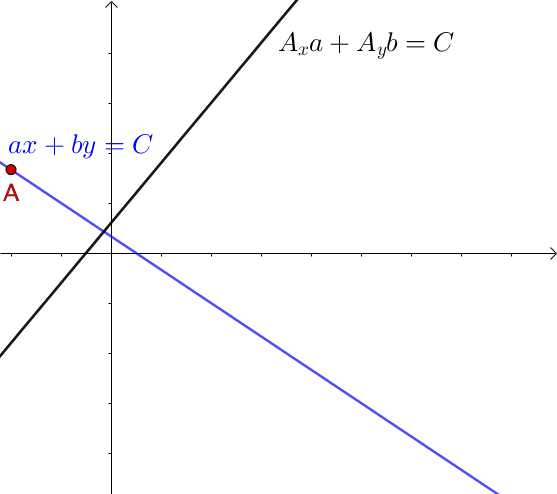
\includegraphics[width=.8\textwidth]{dual3.jpg} \newline
在这个过程中,点$A$在直线$ax + by = C$上运动对应不同的$(A_x,A_y)$,即对应不同的$\overrightarrow{v}$,相应的,有与之对应的$$A_xa + A_yb = C$$ 即不同的映射关系$f$。我们可以认为:\newline
$V = \overrightarrow{v_1},\overrightarrow{v_2},\overrightarrow{v_3} \cdots$ \newline
代表点,而:\newline
$V^* = f_1,f_2,f_3,\cdots$ \newline
代表线。则可以定义$V^*$为$V$的对偶空间。
\subsection{张量的理解}
张量的定义为:
$$T : \underbrace{V^* \times \cdots \times V^*}_{m \ copies} \times \underbrace{V \times \cdots \times V}_{n \ copies} \to \mathbb{R}$$
其中有$r$个来自于$V^*$的参数(函数为参数),有$s$个来自于$V$的参数,这样的张量一般称为$(r,s)$型张量,其空间记为$T_s^r(V)$。\newline
例如:\newline
1.向量空间$V$是$(1,0)$型张量空间$T_0^1(V)$,对于每个向量$\overrightarrow{v} \in V$,为$(1,0)$型张量,将线性映射$f \in V^*$映射到$\mathbb{R}$。\newline
2.向量空间的对偶空间$V^*$为$(0,1)$型张量空间$T_1^0(V)$,即每个线性映射$f \in V^*$是一个$(0,1)$张量,即线性映射$L:V \to \mathbb{R}$。 \newline
3.$(1,1)$型张量为方阵,即对任意$(1,1)$型张量$t$,有$t \in T_1^1(V)$,即为多重线性映射$V^* \times V \to \mathbb{R}$,则$t(\cdot,v)$为一个从$V^*$到$R$的线性映射,又由于$(V^*)^* = V$,所以$V$中的每个矢量都可视为线性函数的线性函数,即$t(f,v)$本质上对应于线性映射$V \to V$,即对应于方阵。反过来,对于一个方阵$A$,它可视为矢量空间$V$到$V$的线性映射,与前面的推理过程类似,可得到它的本质为$V^* \times V \to \mathbb{R}$。 \newline
对于一个方阵而言,它的各项为张量在基底下的坐标。例如:选定$(1,1)$型张量,即方阵$V$,若$V = \mathbb{R}^3$,选取基底为$e_1,e_2,e_3$,其对偶空间$(\mathbb{R}^3)^*$也可相应的确定基底$e^1,e^2,e^3$,于是,所有的张量基底有九个:$$e^i \bigotimes e_j,i = 1,2,3,j = 1,2,3$$ 为一个$3 \times 3$矩阵。\newline
分别记为:\newline
$T_0^1(V) \cong L(V^*,\mathbb{R}) \cong V$ \newline
与 \newline
$T_1^0(V) \cong L(V,\mathbb{R}) \cong V^*$ \newline
以及 \newline
$T_1^1(V) \cong L(V,V)$ \newline
综上所述:\newline
1.$(r,s)$型张量实际上是有$r$个线性函数作为参数,$s$个矢量作为参数的映射到实数的多重线性映射。\newline
2.矢量实际上是$(1,0)$型张量,它是线性映射的线性映射。\newline
3.线性泛函实际上是$(0,1)$型张量,是矢量空间到实数的线性映射。\newline
4.矩阵方阵是$(1,1)$型张量。
\section{张量的特征值}
在线性代数中,对于一个特定的矩阵$A$,它的特征向量$v$经过这个线性变换之后,得到的新向量仍然与原来的$v$保持在同一条直线上,但其长度或方向也许会改变,即:$$Av = \lambda v$$ 推广即可得张量的特征值。
\subsection{几种张量的特征值} 
$H$-特征值:\cite{ding2015generalized}
$$Ax^{m-1} = \lambda x^{[m-1]},x^{[m-1]} = [x_1^{m-1},x_2^{m-1},\cdots,x_n^{m-1}]^T$$
$E$-特征值和$Z$-特征值:
$$Ax^{m-1} = \lambda x,x^Tx = 1$$
$D$-特征值:
$$Ax^{m-1} = \lambda Dx,x^TDx = 1$$
\subsection{对称张量的特征值和特征向量}
取$k$阶对称张量$A \in \mathbb{R}^{n \times \cdots \times n}$,其中对称张量的定义为:对任意的排列$\sigma$,有$a_{j_{\sigma (1)} \cdots j_{\sigma (n)}} = a_{j_1 \cdots j_n}$。$k = 3$时可表示为:\cite{lim2005singular}
$$a_{123} = a_{132} = a_{213} = a_{231} = a_{312} = a_{321}$$
由于
$$A(M_1, \cdots, M_n) := [\sum_{j_1 = 1}^{d_1} \cdots \sum_{j_k = 1}^{d_k} a_{j_1 \cdots j_k}x_{j_1}^{(1)} \cdots x_{j_k}^{(k)}]$$
其中$A = [a_{j_1 \cdots j_k}] \in \mathbb{R}^{d_1 \times \cdots \times d_k}$,$M_1 = [m_{j_1 i_1}^{(1)}] \in \mathbb{R}^{d_1 \times s_1},\cdots,M_k = [m_{j_k i_k}^{(K)}] \in \mathbb{R}^{d_k \times s_k}$。\newline
那么:
$$A(x, \cdots, x) = \sum_{j_1 = 1}^{n} \cdots \sum_{j_n = 1}^{n} a_{j_1 \cdots j_n}x_{j_1} \cdots x_{j_n}$$
为了便于理解,对上述两个式子讨论$k = 2$的情形:
$$
  A =
  \left[
  \begin{matrix}
  a_{11} & a_{12} \\
  a_{21} & a_{22} 
  \end{matrix}
  \right],
  M_1 =
  \left[
  \begin{matrix}
  m_{11}^{(1)} & m_{12}^{(1)} \\
  m_{21}^{(1)} & m_{22}^{(1)}
  \end{matrix}
  \right],
  M_2 =
  \left[
  \begin{matrix}
  m_{11}^{(2)} & m_{12}^{(2)} \\
  m_{21}^{(2)} & m_{22}^{(2)}
  \end{matrix}
  \right]
$$
则:\newline
\begin{equation}
\begin{split} 
	A(M_1,M_2) =& \sum_{j_1 = 1}^{2} \sum_{j_2 = 1}^{2}[a_{j_1 j_2}m_{j_1 i_2}^{(1)}m_{j_2 i_2}^{(2)}]\\
		  	   =& \sum_{j_1 = 1}^{2} [a_{j_1 1}m{j_1 i_1}^{(1)}m_{1 i_2}^{(2)} + a_{j_1 2}m_{j_1 i_1}^{(1)}m_{2 i_2}^{(2)}]\\
           	   =& m_{1 i_2}^{(2)}[a_{11}m_{1 i_1}^{(1)} + a_{21}m_{2 i_1}^{(1)}] + m_{2 i_2}^{(2)}[a_{12}m_{1 i_1}^{(1)} + a_{22}m_{2 i_1}^{(1)}] \\
           	   =& a_{11}m_{1 i_1}^{(1)}m_{1 i_2}^{(2)} + a_{12}m_{1 i_1}^{(1)}m_{2 i_2}^{(2)} + a_{21}m_{2 i_1}^{(1)}m_{1 i_2}^{(2)} + a_{22}m_{2 i_1}^{(1)}m_{2 i_2}^{(2)}
\end{split}
\end{equation}
同理,若$x_1 = (x_1^{(1)},x_2^{(1)}),x_2 = (x_1^{(2)},x_2^{(2)})$,则:\newline
\begin{equation}
\begin{split}
A{(x_1,x_2)} =& \sum_{j_1 = 1}^{2} \sum_{j_2 = 1}^{2}[a_{j_1 j_2}x_{j_1}^{(1)}x_{j_2}^{(2)}]\\
		   =& \sum_{j_1 = 1}^{2} [a_{j_11}x_{j_1}^{(1)}x_1^{(2)} + a_{j_1 2}x_{j_1}^{(1)}x_2^{(2)}]\\
		   =& a_{11}x_1^{(1)}x_1^{(2)} + a_{12}x_1^{(1)}x_2^{(2)} + a_{21}x_2^{(1)}x_1^{(2)} + a_{22}x_2^{(1)}x_2^{(2)}
\end{split}
\end{equation}
并且可以得到:$\nabla_{x_i}A(x_1,\cdots,x_k) = A(x_1,\cdots,x_{i-1},I_{d_i},x_{i+1},\cdots,x_k)$ \newline
由上述可知,$A$定义了一个$k$阶齐次多项式函数:$\mathbb{R}^n \to \mathbb{R}$。适当选取$l^p$-范数,我们可以考虑多线性瑞利商:
$$A(x,\cdots,x)/{{\|x\|}_p^k}$$
利用拉格朗日乘数法$L:\mathbb{R}^n \times \mathbb{R} \to \mathbb{R}$,即:
$$L(x,\lambda) = A(x,\cdots,x) - \lambda(\|x\|_p^k - 1)$$
可以得到: \newline
\begin{equation}
\left\{
\begin{aligned}
\nabla_xL &= \textbf{0}\\
\nabla_{\lambda}L &= 0\\
\end{aligned}
\right.
\end{equation}
由于\newline
\begin{equation}
\left\{
\begin{aligned} 
\nabla_{x_i}A(x_1,\cdots,x_k) &= A(x_1,\cdots,x_{i-1},I_{d_i},x_{i+1},\cdots,x_k)\\
\nabla \|x\|_p &= \frac{\phi_{p-1}(x)}{\|x\|_p^{p-1}}\\
\phi_p(x) = x_p &:= [x_1^p,\cdots,x_n^p]^T. \text{p为偶数}\\
\end{aligned}
\right.
\end{equation}
即可得到:\newline
$$A(I_n,x,\cdots,x) = \lambda\phi_{p-1}(x)$$
其中$\|x\|_p = 1$,按照上式求出的$\lambda$和$x$分别称为张量的$l^p$特征值和与之对应的$l^p$特征向量。\newline
当$k = 2$时,$l^2$特征对可写为:
$$A(I_n,x,\cdots,x) = \lambda x$$
其中$\|x\|_2 = 1$。\newline
当$k$为偶数时,$l^k$特征对可写为:\newline
$$A(I_n,x,\cdots,x) = \lambda x^{k - 1}$$
\bibliographystyle{plain}
\bibliography{mybib}
\end{document}
